\documentclass{article}
\usepackage{listings}
\usepackage{xcolor}
\usepackage{enumitem}
\usepackage{graphicx}
\usepackage{amssymb}
\usepackage{bytefield}
\usepackage{tikz}
\usetikzlibrary{shapes, positioning}
\usepackage{forest}
\usepackage{fancyhdr} % Custom headers/footers
\usepackage{colortbl}
\usepackage[left=0.6in, right=0.6in, top=1in, bottom=0.9in]{geometry}
\usepackage{indentfirst}
\usepackage{changepage, titlesec}
\usepackage{booktabs}
\usepackage{caption} % Allows using \captionof outside float envir
\usepackage{array}
\usepackage{adjustbox} % for adjustwidth
\usepackage{multicol} % for side-by-side columns
\setlength{\parindent}{1.5em} % Set indentation size (optional)
\usepackage{amsmath} % Required for align environment
\usepackage{xepersian}
\settextfont{Vazirmatn FD}
\setlatintextfont{Noto Serif} 


\pagestyle{fancy}     % Enable fancy headers
\fancyhf{}            % Clear default header/footer
\renewcommand{\headrulewidth}{0pt} % Disable default header line

\fancyhead[L]{\rule{\textwidth}{1pt}} % Manually add one line
\fancyfoot[C]{\thepage} % Page number in the center of the footer

\newcommand{\colorbitbox}[3]{%
	\rlap{\bitbox{#2}{\color{#1}\rule{\width}{\height}}}%
	\bitbox{#2}{#3}}
\definecolor{lightcyan}{rgb}{0.84,1,1}
\definecolor{lightgreen}{rgb}{0.64,1,0.71}
\definecolor{lightred}{rgb}{1,0.7,0.71}

\definecolor{codegreen}{rgb}{0,0.6,0}
\definecolor{codegray}{rgb}{0.5,0.5,0.5}
\definecolor{codepurple}{rgb}{0.58,0,0.82}
\definecolor{backcolour}{rgb}{0.95,0.95,0.92}

\lstdefinestyle{mystyle}{
	backgroundcolor=\color{backcolour},   
	commentstyle=\color{codegreen},
	keywordstyle=\color{magenta},
	numberstyle=\tiny\color{codegray},
	stringstyle=\color{codepurple},
	basicstyle=\ttfamily\footnotesize,
	breakatwhitespace=false,         
	breaklines=true,                 
	captionpos=b,                    
	keepspaces=true,                 
	numbers=left,                    
	numbersep=5pt,                  
	showspaces=false,                
	showstringspaces=false,
	showtabs=false,                  
	tabsize=2
}

\lstset{style=mystyle}

\ExplSyntaxOn
\NewDocumentCommand{\ReverseWords}{m}
{
	\seq_set_split:Nnn \l_tmpa_seq { ~ } { #1 } % Split words by spaces
	\seq_reverse:N \l_tmpa_seq % Reverse the order of words
	\seq_use:Nn \l_tmpa_seq { ~ } % Join words with spaces and output
}
\ExplSyntaxOff

\begin{document}
	\title{\huge تکلیف دوم}
	\author{مجتبی ملایی \\ ۴۰۱۳۱۳۸۳}
	\maketitle
	
	
	
\section{P14}
\begin{enumerate}
	\item eBGP
	\item iBGP
	\item eBGP
	\item iBGP
\end{enumerate}

\section{P15}
\begin{enumerate}
	\item 
\lr{l1} .
چون مسیر با کمترین هزینه از \lr{d1} به \lr{c1} از اینترفیس \lr{l1} عبور می‌کند.
	\item 
	\lr{l2}. 
	هر دو مسیر AS-PATH یکسانی دارند. اما مسیری که از \lr{l2} میگذرد، مسیریاب NEXT-HOP نزدیک تری دارد.  
	\item 
	\lr{l1}. 
	زیرا این مسیر AS-PATH کمتری دارد.
\end{enumerate}


\section{P17}



	
\begin{center}
	\begin{minipage}{0.48\textwidth}
		\centering

		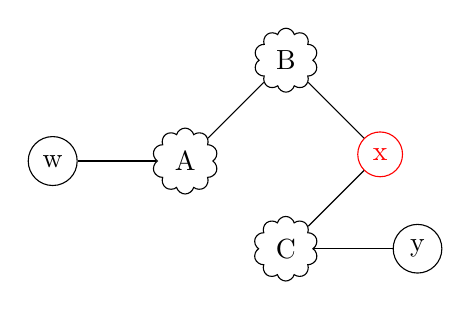
\begin{tikzpicture}
			% Nodes
			\node (w) [circle, draw] {w};
			\node (A) [cloud, draw, right=1cm of w] {A};
			\node (B) [cloud, draw, above right=1cm of A] {B};
			\node (x) [circle, draw, below right=1cm of B, color=red] {x};
			\node (C) [cloud, draw, below left=1cm of x] {C};
			\node (y) [circle, draw, right=1cm of C] {y};
			
			% Edges
			\draw (w) -- (A);
			\draw (A) -- (B);
			\draw (B) -- (x);
			\draw (x) -- (C);
			\draw (C) -- (y);

		\end{tikzpicture}
		\captionof{figure}{\ReverseWords{X's view of network}}
	\end{minipage}
	\hfill
	\begin{minipage}{0.48\textwidth}
		\centering
		
		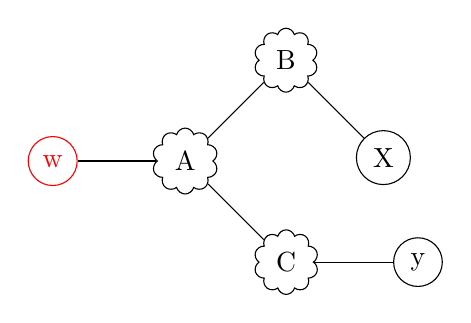
\begin{tikzpicture}
			% Nodes
			\node (w) [circle, draw, color=red] {w};
			\node (A) [cloud, draw, right=1cm of w] {A};
			\node (B) [cloud, draw, above right=1cm of A] {B};
			\node (X) [circle, draw, below right=1cm of B] {X};
			\node (C) [cloud, draw, below right=1cm of A] {C};
			\node (y) [circle, draw, right=1cm of C] {y};
			
			% Edges
			\draw (w) -- (A);
			\draw (A) -- (B);
			\draw (B) -- (X);
			\draw (A) -- (C);
			\draw (C) -- (y);

		\end{tikzpicture}
		\captionof{figure}{\ReverseWords{W's view of network}}
	\end{minipage}
\end{center}
A 
مسیر خود به W را به B و C می‌فرستد اما ‌B و C مسیر AW را طبق قرار داد برای یکدیگر نمی‌فرستند ولی به مشتری هایشان میفرستند. یعنی B مسیر خود به W را ب x می‌میفرستد و C نیز مسیر خود به W را به x و y میفرستد. به طور مشابه C و ‌B نیز مسیر خود را به A میفرستند.
	
	
\section{P19}
A 
باید AV و AW را B تبلیغ کند . اما به C فقط  AV را تبلیغ کند.
C 
مسیر AV را را از A دریافت میکند و مسیر های BAV و ‌BAW را از B دریافت مکیند.  چون A مشتری B به حساب می آید.


\section{P20}

چون Z قرار است دیتای Y را جابه جا کند، بنابراین تمامی مسیر های خود را به Y میفرستد. حالا Y میتواند مسیر هایی که از Z قابل دسترسی هستند را به دیگران از جمله X بفرستد. پس Z نمیتواند چنین کاری بکند.  	
\end{document}







